\PassOptionsToPackage{usenames,dvipsnames,table,x11names}{xcolor}
\documentclass[10pt]{article}

%------------------------------------------------------
%                Math Packages
%------------------------------------------------------

%\usepackage[intlimits]{amsmath}
\usepackage{amsmath}
\usepackage{amssymb}
\usepackage{amsthm}
%\everymath{\displaystyle}
\usepackage{siunitx} % for SI units (e.g. C, degree)
\usepackage{bm} % bold for some math symbols
\usepackage{nicefrac} % for nicer fractions sometimes
\usepackage[thinc]{esdiff} % for derivatives
\usepackage{mathtools}

%------------------------------------------------------
%                Tikz and Pgfplots
%------------------------------------------------------

\usepackage{pgfplots}
\usepackage{tkz-euclide}
\pgfplotsset{compat=1.15}
\usetikzlibrary{arrows,shadows,positioning, calc, decorations.markings, hobby, quotes, angles, decorations.pathreplacing, intersections, matrix,backgrounds}
\usepgfplotslibrary{polar,colormaps,fillbetween}
\usepgflibrary{shapes.geometric}
%\usetkzobj{all}

%------------------------------------------------------
%                Formatting
%------------------------------------------------------

% COLORS ----------------------------------------------
%\usepackage[dvipsnames, table]{xcolor}
\usepackage{xcolor}

% FIGURES ---------------------------------------------
\usepackage{graphicx} % for importing images
\usepackage{subcaption} % for making subfigures
\usepackage[textfont=it]{caption} % changing style of figures
% labelfont=bf % sometimes use this too

% PAGE LAYOUT -----------------------------------------
%\linespread{1.3} % changes line spacing

\usepackage[a4paper, portrait, margin=1in]{geometry} % for changing layout of document
%\usepackage[a4paper, portrait, left=0.75in, right = 0.75in, top = 1in, bottom=1in]{geometry}

%\usepackage{indentfirst}
%\usepackage{parskip} % for not indenting paragraphs first
\usepackage{multirow} % having multiple rows
\usepackage{multicol} % having multiple columns
\renewcommand\labelitemi{$\vcenter{\hbox{\tiny$\bullet$}}$} % making bullets in \enumerate smaller
\usepackage[T1]{fontenc} % can combine \sc and \bf font
\usepackage{pdflscape} % for changing page orientation
%\usepackage[usestackEOL]{stackengine} % something to do with tables

% LINKS -----------------------------------------------
\usepackage{etoolbox}
\makeatletter % <================================================
\patchcmd{\maketitle}%
  {\def\@makefnmark{\rlap{\@textsuperscript{\normalfont\@thefnmark}}}}%
  {\def\@makefnmark{\rlap{\@textsuperscript{\normalfont\color{blue}\@thefnmark}}}}%
  {}%success
  {}%failure
\makeatother % <=================================================
% for changing color of \thanks{} in title

\usepackage[hidelinks]{hyperref}
\hypersetup{
    colorlinks=true,
    linkcolor=black,
    filecolor=magenta,      
    urlcolor=black,
    citecolor=Blue4,
}

% LANGUAGES -------------------------------------------
\usepackage[english]{babel} % for correctly using english
\usepackage[utf8x]{inputenc} % compiling correctly
\usepackage{CJK} % using Chinese, Japanese, and Korean

% MISC ------------------------------------------------
\usepackage[normalem]{ulem} % for \sout
\usepackage{tikzsymbols} % for emojis
\usepackage{booktabs,eqparbox} % for tables
\usepackage{tabularx} % more customizable tables
\usepackage{verbatim} % for verbatim environment

% CITING ----------------------------------------------
\usepackage{apacite}

%------------------------------------------------------
%                Custom Commands
%------------------------------------------------------

\newcommand{\done}{\hfill $\square$}
\newcommand{\csch}{\mathrm{csch}}
\newcommand{\sech}{\mathrm{sech}}

%\newcommand{\dd}{\mathop{}\,\mathrm{d}}
\newcommand{\dd}{\,\mathrm{d}}

% COLOR CODING -----------------------------------------------
\newcommand{\code}[1]{\textcolor{Bittersweet}{\texttt{#1}}} % using for emphasizing variables, code, etc.
\newcommand{\mydef}[1]{\textcolor{SteelBlue3}{\textit{#1}}} % defining something

% VENN DIAGRAMS ----------------------------------------------
\def\firstcircle{(90:1.75cm) circle (2.5cm)}
\def\secondcircle{(210:1.75cm) circle (2.5cm)}
\def\thirdcircle{(330:1.75cm) circle (2.5cm)}
\def\sampspace{(-6,-4.25) rectangle (6,5)}  %Cartesian
%\def\sampspace{(225:7cm) rectangle (45:7cm)} %polar

% TO DO LIST -------------------------------------------------
\usepackage{enumitem}

\newlist{todolist}{itemize}{2}
\setlist[todolist]{label=$\square$}

\usepackage{pifont}
\newcommand{\cmark}{\ding{51}}%
\newcommand{\xmark}{\ding{55}}%
\newcommand{\fin}{\rlap{$\square$}{\raisebox{2pt}{\color{Green}{\large\hspace{1pt}\cmark}}}%
\hspace{-2.5pt}}
\newcommand{\wontfix}{\rlap{$\square$}{\color{red}{\large\hspace{1pt}\xmark}}}

% LADE STUFF -------------------------------------------------
\xdef\defsize{4}
\xdef\cursize{5}
\newcommand{\myscale}[1]{\defsize/#1}

%------------------------------------------------------
%                Custom Environments
%------------------------------------------------------

\usepackage{mdframed}

% EXERCISE -------------------------------------------------
\mdfdefinestyle{exercise}{
	backgroundcolor=black!10,roundcorner=8pt,hidealllines=true,nobreak
}

%\begin{mdframed}[style=exercise]
%\end{mdframed}

% MATHEMATICA ------------------------------------------------
\mdfdefinestyle{mathematica}{
	backgroundcolor=Tan!15,roundcorner=8pt,hidealllines=true,nobreak,fontcolor=Bittersweet
}

% R ---------------------------------------------------------
\mdfdefinestyle{R}{
	backgroundcolor=SteelBlue3!10, roundcorner=8pt, hidealllines=true, fontcolor=SteelBlue4
}

% R ---------------------------------------------------------
\mdfdefinestyle{python}{
	backgroundcolor=Green!15, roundcorner=8pt, hidealllines=true, fontcolor=Green
}

%------------------------------------------------------
%                      Layout
%------------------------------------------------------

% FORMATTING TITLES -----------------------------------
\usepackage{titlesec}
\titleformat*{\section}{\Large \bfseries} % changing section format
\titleformat*{\subsection}{%\color{SteelBlue3} 
\large \bf} % changing subsection format
%\setcounter{secnumdepth}{0} % sets title counter to 0

% PAGE HEADINGS ----------------------------------------------
\usepackage{fancyhdr}

\pagestyle{plain}
\fancyhf{}
\lhead{}
\chead{}
\rhead{}
\cfoot{{ \thepage}}

\renewcommand{\headrulewidth}{0.2pt}
\renewcommand{\footrulewidth}{0pt}
%\pagenumbering{gobble}
\newcommand{\mycc}{\cellcolor{SteelBlue3!10}}

%%%%%%%%%%%%%%%%%%%%%%%%%%%%%%%%%%%%%%%%%%%%%%%%%%%%%%%
%%%%%%%%%%%%%%%%%%%%%%%%%%%%%%%%%%%%%%%%%%%%%%%%%%%%%%%
\begin{document}

%------------------------------------------------------
%                       Title
%------------------------------------------------------

\title{Summary of Regularization Techniques}
\author{Danielle Solomon and Aiden Kenny\\
Lamar University\\
4400 S M L King Jr Pkwy, Beaumont, TX 77705}
\date{Summer 2019}
\maketitle

%------------------------------------------------------
%                      Document
%------------------------------------------------------

NOTES FROM AIDEN:
\begin{itemize}
    \item Look into chapters 7 and 8 in SLS, info about principal components, neural nets, sparse clustering, notation for within-cluster variance pp.230.
\end{itemize}

Title (?): Unsupervised learning to improve prediction accuracy

\section{Introduction}
   
High-dimensional data sets, ones where the number of predictors vastly outnumber the number of observations, present several problems during analysis. It is difficult to take into account the influence of each of the predictors due to the exorbitant amount, and it is often the case that many of the predictors are highly-correlated. From this large pool of predictors, some predictors are more influential than others. Regularization is a useful technique when working with high-dimensional data sets; it aims to introduce a small amount of bias in the model with the hopes of drastically lowering the variance, thus improving prediction accuracy.

Various regression models (e.g. linear and logistic) can be modified by many kinds of penalties which allow different types of regularization to occur. Genome data is an example of real-world data that is used to test these regularization techniques because of its high-dimensional nature. The lasso \cite{tibshirani1996regression} minimizes the loss function with an added $\ell_1$ penalty imposed on the coefficient vector $\bm{\beta}$. If the shrinkage is severe enough, entire coefficients will be set to zero, i.e. the lasso produces \textit{sparse} models. However, there are times when the lasso does not perform well (e.g. when the predictors are highly-correlated); one alternative is the \textit{elastic net} \cite{zou2005regularization}, which imposes a combination of an $\ell_1$ penalty and a squared $\ell_2$ penalty. 

One drawback of the lasso is that it does not take into account any grouping structure within the data, which can often be exploited to improve prediction accuracy. The group lasso (gLasso) \cite{yuan2006model} imposes an $\ell_2$ norm on each of the pre-defined groups. As a result, gLasso imposes sparsity \textit{among} different groups; however, one drawback is that there is no sparsity \textit{within} each group. A compromise is the sparse group lasso (sgLasso) \cite{friedman2010note} combines the lasso and gLasso penalties, and the resulting model will have sparsity both within and among the groups. %This is especially useful in regards to genome data because sparse group lasso is useful in identifying the pathways of interest and and selecting pathways of interest from them. 
%Sparse group lasso also shrinks the estimated effects of driving genes within a group toward one another (Simon et al). 

Principal components lasso (pcLasso) \cite{2018arXiv181004651T} is another method that can be applied both without and with group structure. It applies both an $\ell_1$ penalty on the entire coefficient vector and a ``pcLasso penalty'' to each group. The pcLasso penalty is a quadratic penalty based off of the SVD of each group. For each group, pcLasso shrinks each group vector toward that group's leading principal axis. %PcLasso also is capable of inducing group sparsity, similar to group lasso. However, pcLasso has proven to be more equipped to handle data sets that can be too large for sparse group lasso. 

It is often the case that the groups for a data set are known before the analysis is performed. If the data set has some type of grouping structure that is not known, this grouping structure cannot be exploited to improve prediction accuracy. It is possible to perform \textit{cluster analysis}, an unsupervised learning technique, on the data set an gain an insight on the possible group structure. We can then perform regularization using these groups as the predictors, hopefully improving prediction accuracy. 
%However, there are not many studies that cluster the data before employing these regularization techniques and use the regularization techniques on the entire data set. It is unsure if there is difference in the outcome when using that has been preclustered versus data that is considered as a whole. We are going to compare the prediction accuracy of these different regularization techniques applied to a data set as a whole versus the clustered version of the same data set.

We want to see if applying unsupervised clustering methods to data sets has the ability to improve prediction accuracy. 

\section{Notation}

Here is the default notation and rules we should use for the paper:
\begin{itemize}
    \item \mydef{Scalars}: scalars will always be denoted in italic font, e.g. $a$.
    \item \mydef{Vectors}: two cases:
    \begin{enumerate}
        \item By default, a vector will be written in lowercase, boldface, italic font, e.g. $\bm{a}$.
        \item In special cases, a vector will have length $n$ (e.g. the column vectors of a data matrix). Here the vector will be written in lowercase boldface only, e.g. $\mathbf{a}$.
    \end{enumerate}
    The elements of a vector are denoted as scalars with subscripts, the subscript indicating which element of the vector it is. So $a_2$ is the second element of $\bm{a}$.
    
    By default, vectors are \textit{column vectors}, so $\bm{a} \in \mathbb{R}^p$ is a $p \times 1$ vector, while its transpose $\bm{a}^T$ is a row vector. So 
    \begin{align*}
        \bm{a} = \begin{pmatrix}
            a_1 \\ \vdots \\ a_p
        \end{pmatrix}
        \text{~~~and~~~} 
        \bm{a}^T = \begin{pmatrix}
            a_1 & \cdots & a_p
        \end{pmatrix}.
    \end{align*}
    Will also write vectors in-line as $\bm{a} = (a_i, \ldots, a_p)$.
    \item \mydef{Matrices}: matrices will always be written in capital boldface, e.g. $\mathbf{A}$.
    
    The elements of matrices are represented as scalars with two subscripts, separated by commas; the first subscript indicates the row, and the second subscript indicates the column. So
    \begin{align*}
        \mathbf{A} = \begin{pmatrix}
            a_{1,1} & \cdots & a_{1,p} \\
            \vdots & \ddots & \vdots \\
            a_{n,1} & \cdots & a_{n,p}
        \end{pmatrix}.
    \end{align*}
    Can also write matrices in-line as $\mathbf{A} = \{ a_{i,j} \}$ for $i = 1, \ldots, n$ and $j = 1, \ldots, p$.
    
    For a matrix $\mathbf{A}$, we denote the row vectors as $\bm{a}_i$ and the column vectors as $\mathbf{a}_j$. Note that they are both column vectors. This lets us re-write $\mathbf{A}$ as 
    \begin{align*}
        \mathbf{A} = \begin{pmatrix}
            \bm{a}_1^T \\ \vdots \\ \bm{a}_n^T
        \end{pmatrix}
        = 
        \begin{pmatrix}
            \mathbf{a}_1 & \cdots & \mathbf{a}_p
        \end{pmatrix}.
    \end{align*}
    \item \mydef{Dimensions}: three cases:
    \begin{enumerate}
        \item For scalars, we say $a \in \mathbb{R}$.
        \item For vectors, we denote a $p$-vector $\bm{a} \in \mathbb{R}^{p}$.
        \item For matrices, we denote an $n \times p$ matrix as $\mathbf{A} \in \mathbb{R}^{n \times p}$.
    \end{enumerate}
\end{itemize}

\section{Methodology}
\subsection{Logistic Regression}
Many classification problems are \textit{binary}, meaning the response falls into two classes (e.g. patient lived or died, house sold or not sold, game won or lost). For convenience, we will code the response as $Y \in \{ 0,1 \}$. We wish to model the \textit{probability} that the response falls into either class, given an input $X$. Let $p(\bm{x}) = \mathbb{P}(Y = 1 \mid X = \bm{x})$, and so $1 - p(\bm{x}) = \mathbb{P}(Y = 0 \mid X = \bm{x})$. The response $\mathbf{y} = (y_1, \ldots, y_n)$ is modeled as 
\begin{align*}
    \log \left( \frac{p(\bm{x}_i)}{1 - p(\bm{x}_i)} \right) = \beta_0 + \bm{x}_i^T \bm{\beta}, \\
    y_i = \begin{cases}
        1 & \text{if } p(\bm{x}_i) \ge 0.5 \\
        0 & \text{if } p(\bm{x}_i) < 0.5
    \end{cases}.
\end{align*}
or alternatively, 
\begin{align*}
    p(\bm{x}_i) = \frac{e^{\beta_0 + \bm{x}_i^T \bm{\beta}}}{1 + e^{\beta_0 + \bm{x}_i^T \bm{\beta}}}.
\end{align*}
Here, $\beta_0$ and $\bm{\beta} = (\beta_1, \ldots, \beta_p)$ must be estimated from the data. This is done by minimizing the \textit{negative log-likelihood function}, given by 
\begin{align}
\label{negloglike}
    \mathcal{L}(\beta_0, \bm{\beta}) = - \frac{1}{n} \sum_{i = 1}^n \Big[ y_i\big(\beta_0 + \bm{x}_i^T \bm{\beta}\big) - \log \left(1 + e^{\beta_0 + \bm{x}_i^T \bm{\beta}}  \right) \Big]. 
\end{align}
$\mathcal{L}(\beta_0, \bm{\beta})$ is convex, so it can be optimized efficiently (look into this).


We also will consider fitting the logistic regression model in the group setting. This was introduced in \cite{meier2008group}. Suppose now that the predictors in the data matrix $\mathbf{X}$ are split up into $K$ groups.  

For now, assume that the groups are non-overlapping. If they overlap, the groups have to be re-coded to create non-overlapping groups. Since none of our groups will be overlapping, we will not consider this. Let $p_k$ denote the number of predictors in group $k$. Since we are assuming the groups are overlapping, we have $p_1 + \ldots + p_k = p$, the total number of predictors. Let $\bm{x}_{i,k} \in \mathbb{R}^{p_k}$ denote the vector having information about only the predictors in group $k$. So 
\begin{align*}
    \bm{x}_{i,k} = \begin{pmatrix}
        x_{i,1} \\ \vdots \\ x_{i, p_k}
        \end{pmatrix}
\end{align*}
(not entirely true, but point is to show that only $p_k$ predictors in group $k$ are in this vector), and 
\begin{align*}
    \bm{x}_i = \begin{pmatrix}
    \bm{x}_{i,1}^T & \cdots & \bm{x}_{i,K}^T
    \end{pmatrix}.
\end{align*}
In other words, we are re-writing $\bm{x}_i$ as a vector whose elements are vectors. 
More generally, let $\mathbf{X}_k \in \mathbb{R}^{n \times p_k}$ is the matrix whose columns are the predictors in group $k$. So 
\begin{align*}
    \mathbf{X}_k = \begin{pmatrix}
    \bm{x}_{1,k}^T \\
    \vdots \\
    \bm{x}_{n,k}^T
    \end{pmatrix}
\end{align*}
and 
\begin{align*}
\mathbf{X} = \begin{pmatrix}
\mathbf{X}_1 & \cdots & \mathbf{X}_K
\end{pmatrix} = \begin{pmatrix}
\bm{x}_{1,1}^T & \cdots & \bm{x}_{1,K}^T \\
\vdots & \ddots & \vdots \\
\bm{x}_{n,1}^T & \cdots & \bm{x}_{n,K}^T
\end{pmatrix}.
\end{align*}
Let $\bm{\beta}_k \in \mathbb{R}^{p_k}$ be the sub vector of $\bm{\beta}$ corresponding to group $k$. The goal here is to model $p(\bm{x}_i)$ using the \textit{groups}, $\bm{x}_{i,k}$!
The logistic regression model in the group setting now takes the form 
\begin{align}
    \label{logreggroup}
        \log \left( \frac{p(\bm{x}_i)}{1 - p(\bm{x}_i)} \right) = \beta_0 + \sum_{k=1}^K \bm{x}_{i,k}^T \bm{\beta}_k \triangleq \eta_K(\bm{x}_i).
\end{align}
Now the coefficients are estimating by minimizing the negative log-likelihood function, which now becomes 
\begin{align}
    \label{negloglikegroup}
        \mathcal{L}_K(\beta_0, \bm{\beta}) = - \frac{1}{n} \sum_{i = 1}^n \Big[ y_i\big(\eta_K(\bm{x}_i)\big) - \log \big(1 + e^{\eta_K(\bm{x}_i)}  \big) \Big].
\end{align}


\subsection{K-means Clustering}

\emph{K-means clustering} seeks to partition observations into a pre-specified number of clusters, so that observations within the groups are similar to each other, while observations in different groups are quite different from each other (homogeneous subgroups among the observations). \emph{K} is the pre-specified value of non-overlapping groups. Let $\mathcal{C} = \{ C_{1},..., C_{k} \}$ denote sets containing the indices of observations in each cluster. These sets satisfy two properties:

\begin{enumerate}
    \item $C_{1} \cup C_{2} \cup ... \cup C_{k} = \{1,\ldots,n\}$  (each observation belongs to at least one of $K$ clusters)
    \item $C_{k} \cap C_{k'} = \emptyset  $ for all $k \neq k'$ (no observation belongs to more than one cluster)
\end{enumerate}

For instance, if $i^{th}$ observation is in the $k^{th}$ cluster, $i \in C_{k}$. A good clustering is one for which the within-cluster variation is as small as possible. Within-clustering variation, $W(C_{k})$, is a measure of the amount by which the observations within a cluster differ from each other. The \textit{total within-cluster variation} is the sum of all $W(C_k)$, and chooses the squared Euclidean distance as the dissimilarity measure.
    \begin{align}
    \label{kmeans}
        W(\mathcal{C}) = \sum_{k=1}^K W(C_k) = \sum_{k=1}^K \sum_{i \in C_k} \| \bm{x}_i - \bm{\mu}_k \|_2^2.
    \end{align}
$|C_{k}|$ denotes number of observations in the $k^{th}$ cluster. The within-cluster variation for the $k^{th}$ cluster is the sum of all pairwise squared Euclidean distances between the observations in the $k^{th}$ cluster, divided by the total number of observations in the $k^{th}$ cluster. $K$-means clustering is a ``top-down'' method. We use the GAP statistic \cite{tibshirani2001estimating} to determine the number of clusters. These are both ``hard clustering'' methods, meaning the groups do not overlap. 


\subsection{Hierarchical Clustering}
\emph{Hierarchical clustering} provides an alternate method of clustering data. Unlike $K$-means clustering, hierarchical clustering does not require pre-specified $k$ clusters. It results in a tree-based representation of the observations, known as a dendogram. A dendogram is constructed starting from the leaves and combining clusters up to the trunk. Each leaf of the dendogram represents an observation. When leaves begin to fuse into branches, it indicates that the observations are similar to each other. Branches can fuse with other branches or leaves when moving further up the tree. The height of the fusion indicates how similar or different the observations are. 
Both $K$-means clustering and hierarchical clustering include all the observations in a data set. 

%\newpage

\subsection{Elastic Net}

The \emph{elastic net} was introduced in \cite{zou2005regularization}. It is implemented using the \texttt{R} package \texttt{glmnet}.
Elastic net generalizes lasso and combines it with ridge regression by adding the $\ell_{2}$ penalty to the objective function of the lasso. This method does not utilize the characteristic of being pre-clustered when dealing the predictors. 
    \begin{align*}
     \mathcal{L}(\beta_{0},\bm{\beta}) + \lambda_1 \| \bm{\beta} \|_{1} + \frac{\lambda_2}{2} \|\bm{\beta}\|_{2}^{2}.
    \end{align*}
If $\lambda_1 = 0$, it behaves like ridge regression. If $\lambda_{2} = 0$, it behaves like lasso. Can alternatively be written as 
    \begin{align*}
         \mathcal{L}(\beta_0, \bm{\beta})
    + \lambda \Big[ \alpha \| \bm{\beta} \|_{1} + \frac{1 - \alpha}{2} \|\bm{\beta}\|_{2}^{2} \Big],
    \end{align*}
where $\alpha = \frac{\lambda_1}{\lambda_1 + \lambda_2}$ and $\lambda = \lambda_1 + \lambda_2$. $\alpha = 1$ corresponds to the lasso, while $\alpha = 0$ corresponds to ridge regression. $\alpha \in [0,1]$. This method is preferred, since it controls how much of a ridge and lasso penalty is applied. Can make penalty ``more ridge'' or ``more lasso'' just by tuning $\alpha$. Sometimes both $\hat{\lambda}$ and $\hat{\alpha}$ are estimated from cross validation. However, it is also common to fit a model over a grid of $\alpha$ values and perform cross validation to determine $\lambda$ for each model.

NOTE: this penalty is actually the \textit{na\"{i}ve elastic net penalty} from the original paper. In the paper, the authors suggest scaling the estimated penalty by a factor of $1 + \lambda_1$, since the na\"{i}ve elastic net performs double shrinkage, but in the \texttt{glmnet} documentation there is no mention of this re-scaling occurring.

\vspace{0.5pt}

\subsection{Lasso}

% some useful stuff about lasso
% https://stats.stackexchange.com/questions/17781/derivation-of-closed-form-lasso-solution
% https://stats.stackexchange.com/questions/67736/equivalence-between-elastic-net-formulations?rq=1

The lasso was introduced in \cite{tibshirani1996regression}; the paper mainly focuses on linear regression, but mentions logistic regression (and other generalized linear models) in section 8. They say that using logistic regression, they can no longer center the data to eliminate the intercept $\beta_0$, so look into how this is estimated. 

LASSO, or Least Absolute Shrinkage and Selection Operator, is a regularization technique that shrinks the coefficient estimates to zero. Shrinking the coefficient estimates can significantly reduce variance. The lasso coefficients, $\hat{\beta_{\lambda}^{L}}$, minimize the quantity 
    \begin{align}
    \label{lasso}
         \mathcal{L}(\beta_{0},\bm{\beta}) + \lambda \| \bm{\beta} \|_{1}.
    \end{align}
The penalty is the $l_{1}$ norm $\|\beta\|_{1}$ = $\sum|\beta_{j}|$. The $l_{1}$ penalty has the effect of forcing some of the coefficient estimates to be exactly equal to zero, when the tuning parameter $\lambda$ is sufficiently large. Lasso yields sparse models - models that involve only a subset of the variables. When $\lambda = 0$, lasso gives least squares regression fit. When $\lambda$ is sufficiently large, lasso gives the null model in which all coefficient estimates are equal to zero. Another way to write lasso: we are minimizing $\mathcal{L}(\beta_0, \bm{\beta})$ subject to the constraint
    \begin{align*}
        \lambda \| \bm{\beta} \|_{1} \le \delta,
    \end{align*}
for some constant $\delta$. The goal is to try to find the set of coefficient estimates that lead to the smallest RSS, subject to the constraint that there's a budget $s$  for how large $\| \bm{\beta} \|_1 =  \sum\limits_{j=1}\limits^{P} |\beta_{j}|$ can be. An extremely large $\delta$ gives budget that is not very restrictive, then coefficient estimates can be large. If $s$ is a small value, then $\sum\limits_{j=1}\limits^{p} |\beta_{j}|$ must be small to not violate the budget. 
Cross validation is used to choose the value for $\lambda$ (tuning parameter) or $s$ (constraint).
\begin{itemize}
     \item Choose a grid of $lambda$ values and compute the cross-validation error for each value.
     \item Select tuning parameter value for which the cross-validation error is the smallest. 
\end{itemize}



%\newpage

\subsection{Group Lasso}

The group lasso was originally introduced in \cite{yuan2006model}. Later on, the case of overlapping groups was introduced in \cite{jacob2009group}, but since none of our groups are overlapping, we will not consider it here. 

Predictors belong to predefined groups. Group Lasso is used to shrink and select the members of a group together. $p$ predictors are divided into $L$ groups, with $p_{l}$ being the number of groups in $l$. Matrix $\mathbf{X}_{l}$ represents predictors corresponding to the $l^{th}$ group, with corresponding coefficient vector $\beta_{l}$ Group Lasso minimizes
    \begin{align}
    \label{glasso}
         \mathcal{L}_K(\beta_0, \bm{\beta}) + \lambda \sum_{k=1}^K \| \bm{\beta}_k \|_2.
    \end{align}
It is standard to multiply each $\| \bm{\beta}_k \|_2$ in the left sum by $\sqrt{p_k}$ in order to scale for the group size. A lot of authors left it out, so we will too. $\| \cdot \|_2$ is the Euclidean norm, NOT squared. The Euclidean norm of $\bm{\beta}_k$ is $0$ only if ALL its components are $0$.
\begin{itemize}
    \item This procedure encourages sparsity on group and individual levels.
\end{itemize}
For some values of $\lambda$, an entire group if predictors may drop out.
One drawback is that this sparsity occurs ONLY on the group level.



\subsection{Sparse Group Lasso}
Sparse Group Lasso differs from Group Lasso because Group Lasso does not provide sparsity of groups and sparsity \emph{within} groups. Sparse Group Lasso minimizes
    \begin{align}
    \label{sglasso}
        \mathcal{L}_K(\beta_0, \bm{\beta}) + \lambda \left[ \alpha \| \bm{\beta} \|_1  + \frac{1 - \alpha}{2} \sum_{k=1}^K \| \bm{\beta}_k \|_2 \right].
    \end{align}
$\alpha \in [0,1]$ -  a convex combination of the lasso and group lasso penalties
\begin{enumerate}
    \item $\alpha = 0$ gives group lasso fit
    \item $\alpha = 1$ gives a lasso fit
    \item In the case of no group structure, this reduces to the lasso? Verify from paper.
\end{enumerate}
Group-wise Sparsity: the number of groups with at least one nonzero coefficient. Within Group Sparsity: the number of nonzero coefficients within each nonzero group. Overall Sparsity: the total number of nonzero coefficients irregardless of grouping. It looks similar to elastic net penalty, but it is different because $\|\cdot\|_{2}$ is not differentiable at $0$, so some groups are completely zeroed out. Within each nonzero group it gives an elastic net fit through the $\|\cdot\|_{2}$ penalty parameter a function of the optimal $\|\hat{\bm{\beta}_{k}}\|_{2}$. $\hat{\beta}$ is the value that minimizes the equation.On a group sparsity level, group lasso and sparse group lasso act similarly but sparse group lasso adds uni-variate shrinkage before checking if a group is nonzero. Sparse group lasso takes into account the likelihood of some levels of predictors being uninformative as the number of levels per predictors increases - sparse group lasso sets the coefficients for many levels to $0$, even in nonzero groups. Sparse group lasso is useful when used on data where the predictors have a natural grouping. Regarding genomic data, sparse group lasso is useful in finding pathways of interest and selects driving genes from them. It shrinks the estimated effects of driving genes within a group toward one another.

%\newpage

\subsection{Principal Component Lasso}

Principal components lasso (pcLasso) was introduced in \cite{2018arXiv181004651T}. We will first consider the non-group setting. 

PcLasso is suited for data where the number of predictors is much greater than the number of observations. $\mathbf{X}$ is the $n$ x $p$ matrix ($n$ observations, $p$ predictors). Let $\mathbf{X} = \mathbf{U} \mathbf{D} \mathbf{V}^T$ be the economy singular value decomposition (SVD) of $\mathbf{X}$. When we say economy, we mean:
\begin{itemize}
    \item $\mathbf{U} \in \mathbb{R}^{n \times p}$
    \item $\mathbf{D} \in \mathbb{R}^{p \times p}$ where $\mathbf{D} = \mathrm{diag}(d_1, \ldots, d_p)$ contain the singular values in descending order. 
    \item $\mathbf{V} \in \mathbb{R}^{p \times p}$.
\end{itemize}
   
Given pre-existing groups, pcLasso shrinks each group-wise component of the solution toward the leading principal components of that group - it also carries out selection of the feature groups.
Let 
\begin{align*}
    \mathbf{D}_{d_1^2 - d_j^2} = \mathrm{diag}(d_1^2 - d_1^2, \ldots, d_1^2 - d_p^2)
\end{align*}
be the pcLasso penalty matrix. PcLasso minimizes the function 
\begin{align}
\label{pclasso}
\mathcal{L}(\beta_0, \bm{\beta}) + \lambda \| \bm{\beta} \|_1 + \frac{\theta}{2} \bm{\beta}^T \mathbf{V} \mathbf{D}_{d_1^2 - d_j^2} \mathbf{V}^T \bm{\beta}.
\end{align}
The objective function is convex - solutions can be found efficiently even for large values of $n$ and $p$. $\beta$ is the vector containing $p$ coefficient estimates. It combines the lasso sparsity penalty with a quadratic penalty that shrinks the coefficient vector towards the leading principal components of the feature matrix. The purpose of this penalty is to impose a weak penalty in the direction of the first principal component, and impose a subsequently stronger penalty in the direction of the weaker principal components. As a result, the estimated coefficients are more likely to lie in the direction of the leading principal component, leading to better prediction accuracy. It strongly biases the solution vector toward the leading singular vectors.
Now for the group setting:
Let $\mathbf{X}_k = \mathbf{U}_k \mathbf{D}_k \mathbf{V}_k^T$ be the SVD of the matrix for the $k$th group, $\mathbf{X}_k$. PcLasso in the group setting minimizes 
\begin{align}
\label{pclassogroup}
\mathcal{L}_K(\beta_0, \bm{\beta}) + \lambda \| \bm{\beta} \|_1 + \frac{\theta}{2} \sum_{k=1}^K \bm{\beta}_k^T \big( \mathbf{V}_k \mathbf{D}_{d_{k,1}^2 - d_{k,j}^2} \mathbf{V}_k^T \big) \bm{\beta}_k.
\end{align}
($\mathbf{V}_k, d_k)$ right singular vectors and singular values of $\mathbf{X}_k$. $\beta_k$ is the subvector of $\beta$ corresponding to group $k$. $d_k = (d_{k1},...,d_{km})$ singular values of $\mathbf{X}_k$ in decreasing order. $\mathbf{D}_{d^2_{k1}-d^2_{kj}}$ diagonal matrix with diagonal entries ${d^2_{k1}-d^2_{kj}}$ for $j=1,2,...,m_k$.
The approach to solving this is to fix a few values of $\theta$ and then optimize the equation over a path of $\lambda$ values. If $\theta = 0$, it becomes equivalent to lasso. 
    
\section{Contour Plots}

\begin{figure}
    \centering
    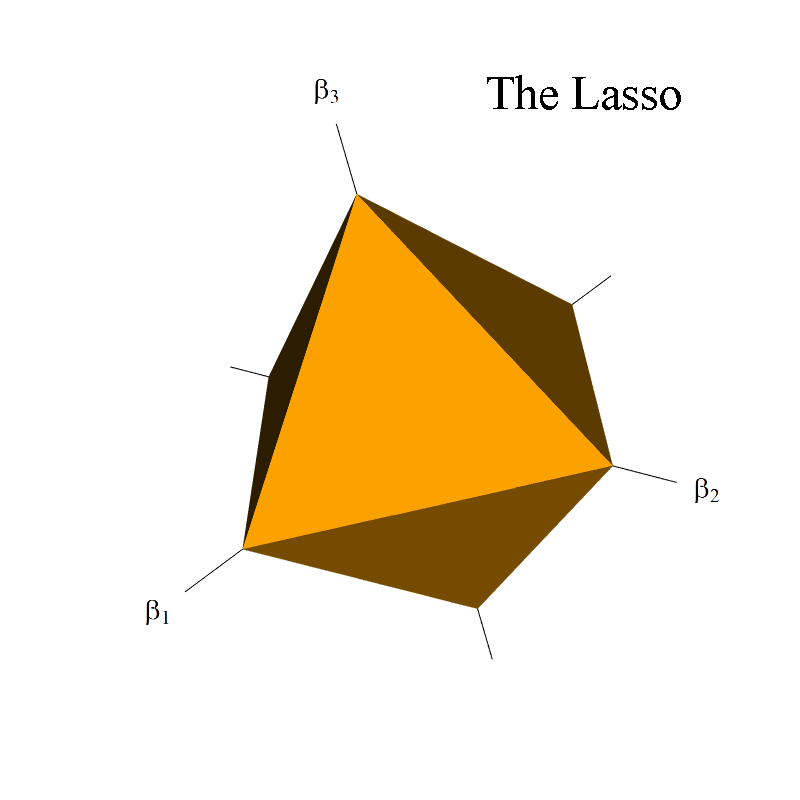
\includegraphics[width = 0.32\textwidth]{3D_lasso_contour.png}
    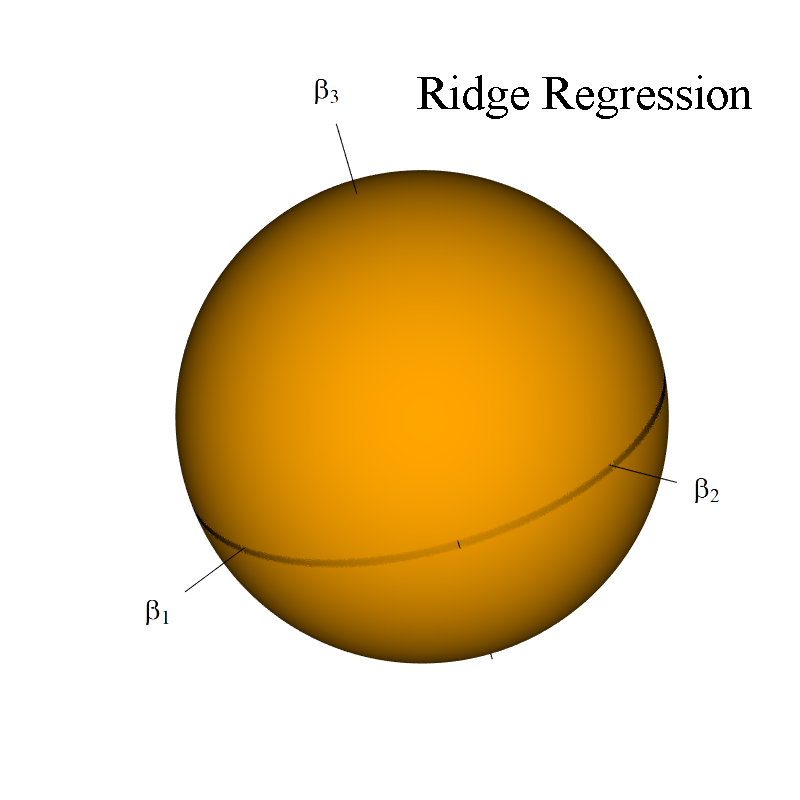
\includegraphics[width = 0.32\textwidth]{3D_ridge_contour.png}
    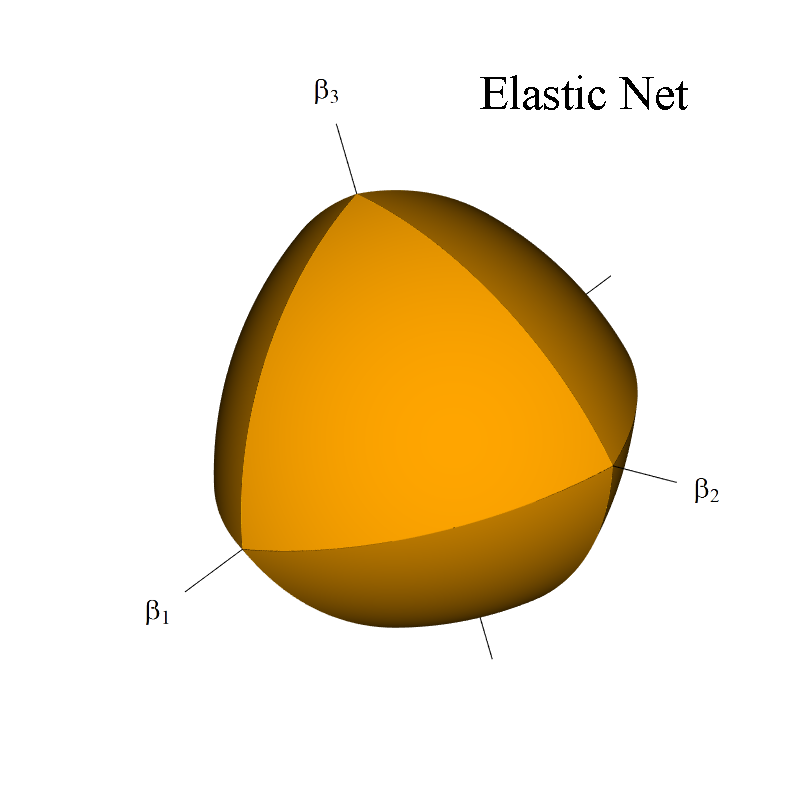
\includegraphics[width = 0.32\textwidth]{3D_enet_contour.png}
    
    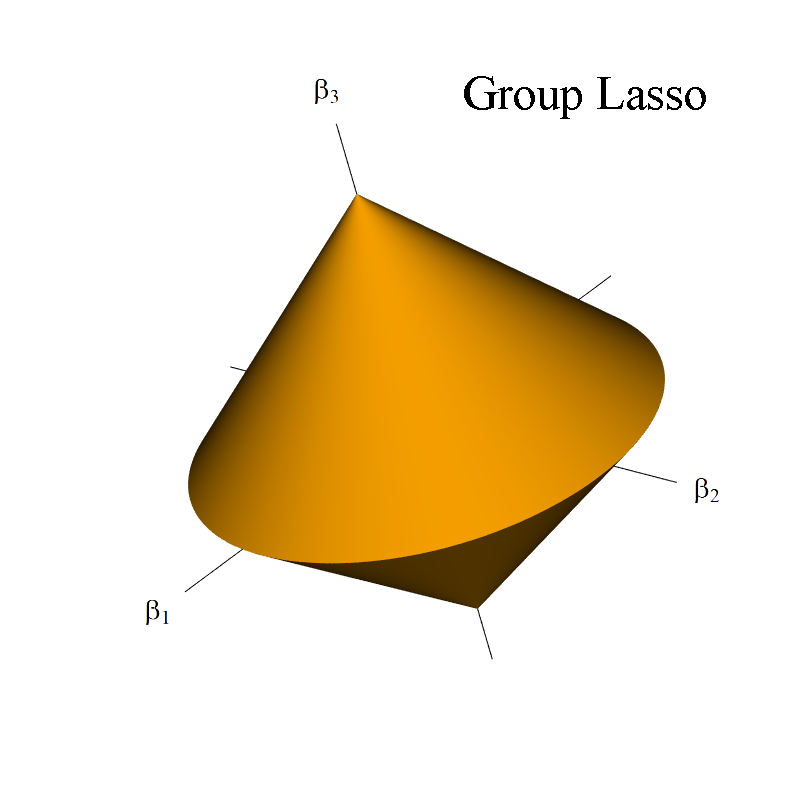
\includegraphics[width = 0.32\textwidth]{3D_glasso_contour.png}
    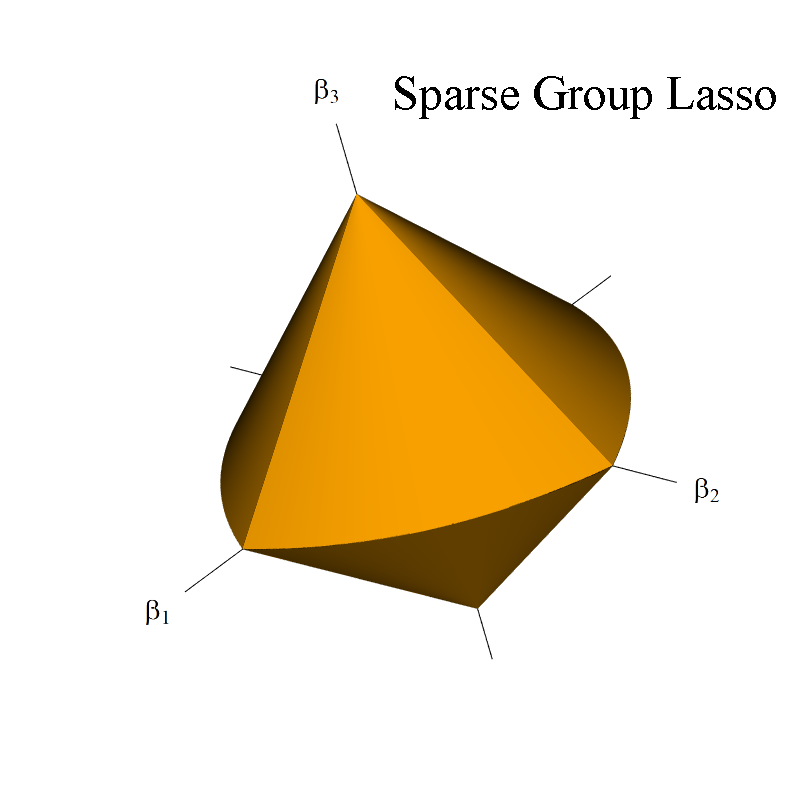
\includegraphics[width = 0.32\textwidth]{3D_sglasso_contour.png} \hspace{0.2cm}
    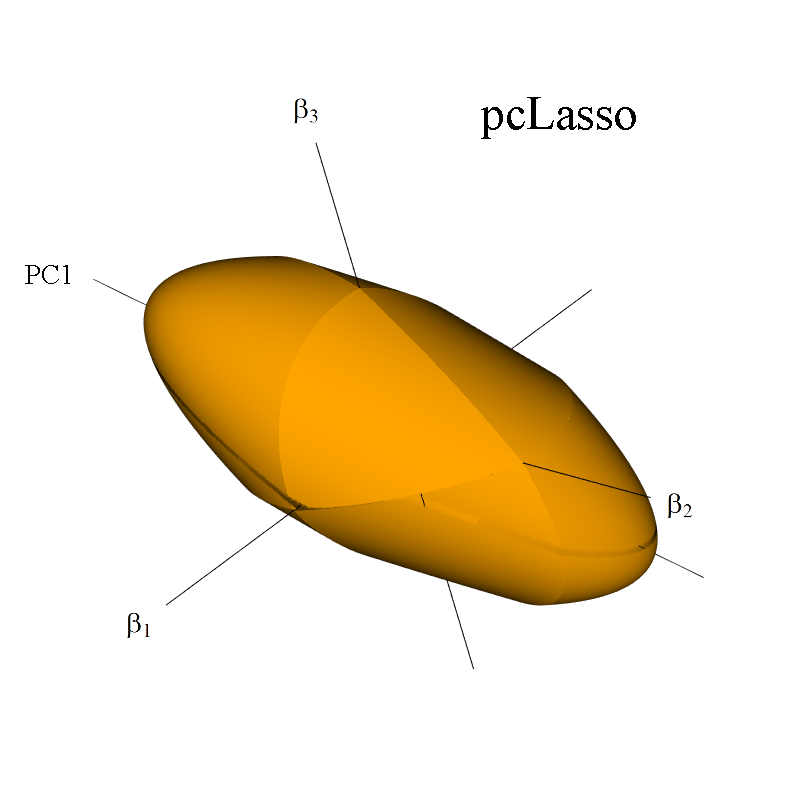
\includegraphics[width = 0.32\textwidth]{3D_pclasso_contour3.png}
    \caption{Comparing the 3-dimensional contour balls for various regularization techniques.}
    \label{groupcontours}
\end{figure}

%\newpage

\section{Generalizations}
\begin{itemize}
    \item In the non-group setting, the most general regularization technique, the $\mathbf{Z}$ penalty, is given my \textit{minimizing} the function 
    \begin{align*}
        J = \mathcal{L}(\beta_0, \bm{\beta}) + \lambda \| \bm{\beta} \|_1 + \frac{\theta}{2} \bm{\beta}^T \mathbf{V} \mathbf{Z} \mathbf{V}^T \bm{\beta}.
    \end{align*}
    \item We can see that:
    \begin{enumerate}
        \item This penalty reduces to the \textit{elastic net} when $\mathbf{Z} = \mathbf{I}$.
        \item This penalty reduces to the \textit{pcLasso} when $\mathbf{Z} = \mathbf{D}_{d_1^2 - d_j^2}$.
        \item $\theta = 0$ corresponds to the lasso. 
    \end{enumerate}

    \item In the group lasso, \cite{yuan2006model} consider a more general penalty 
    \begin{align*}
        \mathcal{L}_K(\beta_0, \bm{\beta}) + \lambda \sum_{k=1}^K \sqrt{\bm{\beta}^T \mathbf{R}_k \bm{\beta}}.
    \end{align*}
    \begin{itemize}
        \item Here, $\mathbf{R}_k$ is a penalty matrix for group $k$.
        \item The normal group lasso chooses $\mathbf{R}_1 = \ldots = \mathbf{R}_K = \mathbf{I}$ ( or $\sqrt{p_k} \mathbf{I}$).
        \item The standardized group lasso chooses $\mathbf{R}_k = \mathbf{X}_k^T \mathbf{X}_k$ (have too look into this more). The standardized group lasso was introduced in \cite{simon2012standardization}. In their original paper, the group lasso, the data matrices were designed to be orthogonal, i.e. $\mathbf{X}_k^T = \mathbf{X}_k$ for all $k$. What \texttt{R} packages implement this?
    \end{itemize}
    \item Then the generalization of the sparse group lasso is 
    \begin{align*}
        \mathcal{L}_K(\beta_0, \bm{\beta}) + \lambda \| \bm{\beta} \|_1 + \theta \sum_{k=1}^K \sqrt{\bm{\beta}^T \mathbf{R}_k \bm{\beta}} = \mathcal{L}_K(\beta_0, \bm{\beta}) + \lambda \| \bm{\beta} \|_1 + \theta \sum_{k=1}^K \| \mathbf{R}_k^{1/2} \bm{\beta} \|_2.
    \end{align*}
\end{itemize}

%------------------------------------------------------
%                      References
%------------------------------------------------------

\bibliographystyle{apacite}
\bibliography{summaries}

\section{Layout of Paper?}

Here is an outline of the format of the paper:
\begin{enumerate}
    \item Introduction
    \begin{itemize}
        \item Talk about the general problem we are trying to solve -- high dimensional classification. 
        \begin{itemize}
            \item Prediction accuracy
            \item Interpretive model
            \item Does performing shrinkage on clusters improve prediction accuracy?
        \end{itemize}
        \item Give formulas for logistic regression, both original and group.
        \item Maybe briefly talk about notation?
    \end{itemize}
    \item Regularization techniques
    \begin{itemize}
        \item The lasso
        \item Briefly mention ridge regression
        \item Elastic net
        \item Talk about problems with each method, and how elastic net seeks to overcome them. 
        \item pcLasso -- have to talk about SVD, and explain motivation behind it
        \item Contour plots! One for lasso, elastic net, and pcLasso.
        \item Maybe mention generalization?
    \end{itemize}
    \item The group setting.
    \begin{itemize}
        \item Group lasso
        \item Problems with group lasso -- only has sparsity among groups, original papers required $\mathbf{X}_k$ to be orthonormal. 
        \item To over come this: sparse group lasso, standardized group lasso. 
        \item Talk about benefits and drawbacks of each, e.g. computational considerations.
        \item pcLasso extends to the group setting as well. 
        \item Contour plots! One for lasso, group lasso, and sparse group lasso. 
        \item Mention various clustering methods, e.g. K-means, hierarchical, spectral. Look through ESL to see.
    \end{itemize}
    \item Real data examples
    \begin{itemize}
        \item Two data sets: colon data and leukemia data. Explain each data set.
        \item Should look to analyze these data sets for properties. Could help explain why some models perform better than others.           
        \begin{itemize}
            \item Make plots of singular values?
        \end{itemize}
        \item Compare different results depending on model -- non-group:
        \begin{itemize}
            \item \mydef{The lasso}, use \verb|lambda.min| and \verb|lambda.1se| from cross-validation. 
            \item \mydef{The elastic net}, test over grid of values $\alpha = \verb|c(1, 0.8, 0.6, 0.4, 0.2, 0)|$. Take lowest error (?) and use \verb|lambda.min| and \verb|lambda.1se| from cross-validation.
            \item \mydef{pcLasso}: test over grid of values $\verb|ratio| = \verb|c(1, 0.95, 0.9, 0.75, 0.5, 0.25)|$. Take lowest error (?) and use \verb|lambda.min| and \verb|lambda.1se| from cross-validation.
            \item Compare test error rate and number of non-zero coefficients.
            \item Make plot of test error over path index.
            \item AOC charts.
        \end{itemize}
        \item Compare results depending on model: group:
        \begin{itemize}
            \item \mydef{Group Lasso}: use \verb|lambda.min| and \verb|lambda.1se| from cross-validation. Implemented with the \texttt{gglasso} package.
            \item \mydef{Standardized group lasso}: look into this, do similar stuff. Implemented with the \texttt{grpreg} package. 
            \item \mydef{Sparse group lasso}: using the \texttt{SGL} package. There does not seem to be way to extract number of nonzero coefficients. Also, lambda index is from $1:20$, not $1:100$ like other packages. 
            \item \mydef{pcLasso}: easy to implement as before.
            \item Compare number of nonzero coefficients and test error. 
            \item Do this for different clustering methods. 
        \end{itemize}
    \end{itemize}
    \item Simulated study
    \item Discussion
\end{enumerate}



%------------------------------------------------------
%                        Tables
%------------------------------------------------------

\newpage

%%%%%%%%%%%%%%%%%%%%%%%%%%%%%%%%%%%%%%%%%%%%%%%%%%%%%%%%%%%%%%%%%%%%%%
%%% ORIGINAL TABLE
%%%%%%%%%%%%%%%%%%%%%%%%%%%%%%%%%%%%%%%%%%%%%%%%%%%%%%%%%%%%%%%%%%%%%%

%\begin{landscape}

%\section{Tables}

%\begin{table}[ht]
%    \centering
%    \def\arraystretch{1.5}
    
%    \begin{tabularx}{0.874\linewidth}{lccccccccc} \toprule
%        & \multicolumn{3}{c}{No Clustering} & \multicolumn{3}{c}{$K$-means Clustering} & \multicolumn{3}{c}{Hierarchical Clustering} \\
%        & \multicolumn{3}{c}{--} & \multicolumn{3}{c}{$K=2$} & \multicolumn{3}{c}{$K=7$} \\ \cmidrule(r){2-4} \cmidrule(lr){5-7} \cmidrule(l){8-10}
%        & Lasso & Elastic Net & pcLasso & gLasso & sgLasso & pcLasso & gLasso & sgLasso & pcLasso \\ \midrule
%        \multirow{2}{*}{Tuning Parameters} & $\lambda =  0.064$ & $\lambda = 0.37$ & $\lambda = 8.75$ & $\lambda = 31.70$ & $\lambda = 0.011$ & $\lambda = 16.78$ & $\lambda = 24.81$ & $\lambda = 0.059$ & $\lambda = 163.94$ \\
%         & -- & $\alpha = 0.2$ & $\texttt{rat} = 0.95$ & -- & $\alpha = 0.4$ & $\texttt{rat} = 0.95$ & -- & $\alpha = 1$ & $\texttt{rat} = 0.95$ \\
%        Misclassifications & $6/31$ & $5/31$ & $5/31$ & $6/31$ & $5/31$ & $4/31$ & $5/31$ & $11/31$ & $3/31$ \\
%        Non-zero Coefficients & $16$ & $63$ & $30$ & $93$ & $66$ & $43$ & $687$ & $1$ & $7$ \\
%        Non-zero Groups & -- & -- & -- & $1$ & $1$ & $2$ & $1$ & $0$ & $4$ \\ \bottomrule
%    \end{tabularx}
%    \caption{The performance of various models on the colon data set.}
%    \label{colontable}
    
%    \vspace{0.45cm} % max is 0.49cm, 0.5cm causes page break
    
%   \begin{tabularx}{0.881\linewidth}{lccccccccc} \toprule
%         & \multicolumn{3}{c}{No Clustering} & \multicolumn{3}{c}{$K$-means Clustering} & \multicolumn{3}{c}{Hierarchical Clustering} \\ 
%         & \multicolumn{3}{c}{--} & \multicolumn{3}{c}{$K=2$} & \multicolumn{3}{c}{$K=5$} \\   
%         \cmidrule(r){2-4} \cmidrule(lr){5-7} \cmidrule(l){8-10}
%         & Lasso & Elastic Net & pcLasso & gLasso & sgLasso & pcLasso & gLasso & sgLasso & pcLasso \\ \midrule
%        \multirow{2}{*}{Tuning Parameters} & $\lambda = 0.0041$ & $\lambda = 0.0051$ & $\lambda = 0.0055$ & $\lambda = 0.017$ & $\lambda = 0.068$ & $\lambda = 0.0055$ & $\lambda = 0.015$ & $\lambda = 0.068$ & $\lambda = 0.0055$ \\ 
%         & -- & $\alpha = 0.8$ & $\texttt{rat} = 1$ & -- & $\alpha = 1$ & $\texttt{rat} = 1$ & -- & $\alpha = 1$ & $\texttt{rat} = 1$ \\ %\addlinespace
%        Misclassifications & $5/36$ & $3/36$ & $2/36$ & $5/36$ & $14/36$ & $2/36$ & $4/36$ & $14/36$ & $2/36$ \\
%        Non-zero Coefficients & $14$ & $28$ & $16$ & $7129$ & $1$ & $16$ & $2714$ & $1$ & $16$ \\
%        Non-zero Groups & -- & -- & -- & $2$ & $1$ & $2$ & $2$ & $1$ & $4$ \\ \bottomrule
%    \end{tabularx}
%    \caption{The performance of various models on the leukemia data set.}
%    \label{leuktable}
    
    %0.7865\linewidth seems fine
    
%\end{table}


%\end{landscape}

%%%%%%%%%%%%%%%%%%%%%%%%%%%%%%%%%%%%%%%%%%%%%%%%%%%%%%%%%%%%%%%%%%%%%%
%%% DUPLICATE TABLE
%%%%%%%%%%%%%%%%%%%%%%%%%%%%%%%%%%%%%%%%%%%%%%%%%%%%%%%%%%%%%%%%%%%%%%

%\newpage

%\begin{landscape}

%\begin{table}[ht]
%    \centering
%    \def\arraystretch{1.5}
    
%    \begin{tabularx}{0.874\linewidth}{lccccccccc} \toprule
%        & \multicolumn{3}{c}{No Clustering} & \multicolumn{3}{c}{$K$-means Clustering} & \multicolumn{3}{c}{Hierarchical Clustering} \\
%        & \multicolumn{3}{c}{--} & \multicolumn{3}{c}{$K=2$} & \multicolumn{3}{c}{$K=7$} \\ \cmidrule(r){2-4} \cmidrule(lr){5-7} \cmidrule(l){8-10}
%        & Lasso & Elastic Net & pcLasso & gLasso & sgLasso & pcLasso & gLasso & sgLasso & pcLasso \\ \midrule
%        \multirow{2}{*}{Tuning Parameters} & $\lambda =  0.064$ & $\lambda = 0.37$ & $\lambda = 8.75$ & $\lambda = 31.70$ & $\lambda = 0.011$ & $\lambda = 8.75$ & $\lambda = 24.81$ & $\lambda = 0.059$ & $\lambda = 8.75$ \\
%         & -- & $\alpha = 0.2$ & $\texttt{rat} = 1$ & -- & $\alpha = 0.4$ & $\texttt{rat} = 1$ & -- & $\alpha = 1$ & $\texttt{rat} = 1$ \\
%        Misclassifications & $6/31$ & $5/31$ & $6/31$ & $6/31$ & $5/31$ & $6/31$ & $5/31$ & $11/31$ & $6/31$ \\
%        Non-zero Coefficients & $16$ & $63$ & $20$ & $93$ & $66$ & $20$ & $687$ & $1$ & $20$ \\
%        Non-zero Groups & -- & -- & -- & $1$ & $1$ & $2$ & $1$ & $0$ & $6$ \\ \bottomrule
%    \end{tabularx}
%    \caption{The performance of various models on the colon data set.}
%    \label{colontable2}
    
%    \vspace{0.45cm} % max is 0.49cm, 0.5cm causes page break
    
%   \begin{tabularx}{0.881\linewidth}{lccccccccc} \toprule
%         & \multicolumn{3}{c}{No Clustering} & \multicolumn{3}{c}{$K$-means Clustering} & \multicolumn{3}{c}{Hierarchical Clustering} \\ 
%         & \multicolumn{3}{c}{--} & \multicolumn{3}{c}{$K=2$} & \multicolumn{3}{c}{$K=5$} \\   
%         \cmidrule(r){2-4} \cmidrule(lr){5-7} \cmidrule(l){8-10}
%         & Lasso & Elastic Net & pcLasso & gLasso & sgLasso & pcLasso & gLasso & sgLasso & pcLasso \\ \midrule
%        \multirow{2}{*}{Tuning Parameters} & $\lambda = 0.0041$ & $\lambda = 0.0051$ & $\lambda = 0.0055$ & $\lambda = 0.017$ & $\lambda = 0.068$ & $\lambda = 0.0055$ & $\lambda = 0.015$ & $\lambda = 0.068$ & $\lambda = 0.0055$ \\ 
%         & -- & $\alpha = 0.8$ & $\texttt{rat} = 0.95$ & -- & $\alpha = 1$ & $\texttt{rat} = 0.95$ & -- & $\alpha = 1$ & $\texttt{rat} = 0.95$ \\ %\addlinespace
%        Misclassifications & $5/36$ & $3/36$ & $2/36$ & $5/36$ & $14/36$ & $2/36$ & $4/36$ & $14/36$ & $2/36$ \\
%        Non-zero Coefficients & $14$ & $28$ & $16$ & $7129$ & $1$ & $62$ & $2714$ & $1$ & $46$ \\
%        Non-zero Groups & -- & -- & -- & $2$ & $1$ & $2$ & $2$ & $1$ & $5$ \\ \bottomrule
%    \end{tabularx}
%    \caption{The performance of various models on the leukemia data set.}
%    \label{leuktable2}
    
    %0.7865\linewidth seems fine
    
%\end{table}


%\end{landscape}

%%%%%%%%%%%%%%%%%%%%%%%%%%%%%%%%%%%%%%%%%%%%%%%%%%%%%%%%%%%%%%%%%%%%%%
%%% NEW TABLE
%%%%%%%%%%%%%%%%%%%%%%%%%%%%%%%%%%%%%%%%%%%%%%%%%%%%%%%%%%%%%%%%%%%%%%

%\newpage

%\begin{landscape}

%\begin{table}[ht]
%    \centering
%    \def\arraystretch{1.5}
    
%   \begin{tabularx}{0.88\linewidth}{lccccccccc} \toprule
%        & \multicolumn{3}{c}{No Clustering} & \multicolumn{3}{c}{$K$-means Clustering} & \multicolumn{3}{c}{Hierarchical Clustering} \\
%        & \multicolumn{3}{c}{--} & \multicolumn{3}{c}{$K=2$} & \multicolumn{3}{c}{$K=7$} \\ \cmidrule(r){2-4} \cmidrule(lr){5-7} \cmidrule(l){8-10}
%        & Lasso & Elastic Net & pcLasso & gLasso & sgLasso & pcLasso & gLasso & sgLasso & pcLasso \\ \midrule
%        \multirow{2}{*}{Tuning Parameters} & $\lambda =  0.064$ & $\lambda = 0.37$ & $\lambda = 8.75$ & $\lambda = 31.70$ & $\lambda = 0.0093$ & $\lambda = 16.78$ & $\lambda = 24.81$ & $\lambda = 0.019$ & $\lambda = 163.94$ \\
%         & -- & $\alpha = 0.2$ & $\texttt{rat} = 0.95$ & -- & $\alpha = 0$ & $\texttt{rat} = 0.95$ & -- & $\alpha = 0$ & $\texttt{rat} = 0.95$ \\
%        Misclassifications & $6/31$ & $5/31$ & $5/31$ & $6/31$ & $5/31$ & $4/31$ & $5/31$ & $11/31$ & $3/31$ \\
%        Deviance & $0.94$ & $1.023$ & $0.56$ & $0.81$ & $1.69$ & $0.54$ & $0.78$ & $1.73$ & $0.55$ \\
%        Non-zero Coefficients & $16$ & $63$ & $30$ & $93$ & $93$ & $43$ & $687$ & $472$ & $7$ \\
%        Non-zero Groups & -- & -- & -- & $1$ & $1$ & $2$ & $1$ & $1$ & $4$ \\ \bottomrule
%    \end{tabularx}
%    \caption{The performance of various models on the colon data set.}
%    \label{colontablenew}
    
%    \vspace{0.45cm} % max is 0.49cm, 0.5cm causes page break
    
%   \begin{tabularx}{0.881\linewidth}{lccccccccc} \toprule
%         & \multicolumn{3}{c}{No Clustering} & \multicolumn{3}{c}{$K$-means Clustering} & \multicolumn{3}{c}{Hierarchical Clustering} \\ 
%         & \multicolumn{3}{c}{--} & \multicolumn{3}{c}{$K=2$} & \multicolumn{3}{c}{$K=5$} \\   
%         \cmidrule(r){2-4} \cmidrule(lr){5-7} \cmidrule(l){8-10}
%         & Lasso & Elastic Net & pcLasso & gLasso & sgLasso & pcLasso & gLasso & sgLasso & pcLasso \\ \midrule
%        \multirow{2}{*}{Tuning Parameters} & $\lambda = 0.0041$ & $\lambda = 0.0051$ & $\lambda = 0.0055$ & $\lambda = 0.0029$ & $\lambda = 0.030$ & $\lambda = 0.0055$ & $\lambda = 0.0030$ & $\lambda = 0.024$ & $\lambda = 0.0055$ \\ 
%         & -- & $\alpha = 0.8$ & $\texttt{rat} = 1$ & -- & $\alpha = 0.8$ & $\texttt{rat} = 0.95$ & -- & $\alpha = 0.4$ & $\texttt{rat} = 0.95$ \\ %\addlinespace
%        Misclassifications & $5/36$ & $3/36$ & $2/36$ & $3/36$ & $14/36$ & $2/36$ & $3/36$ & $14/36$ & $2/36$ \\
%        Deviance & $0.24$ & $0.083$ & $0.45$ & $0.28$ & $1.46$ & $0.44$ & $0.28$ & $1.46$ & $0.44$ \\
%      Non-zero Coefficients & $14$ & $28$ & $16$ & $7129$ & $729$ & $62$ & $2714$ & $772$ & $46$ \\
%       Non-zero Groups & -- & -- & -- & $2$ & $1$ & $2$ & $2$ & $1$ & $5$ \\ \bottomrule
%   \end{tabularx}
%    \caption{The performance of various models on the leukemia data set.}
%    \label{leuktablenew}
    
    %0.7865\linewidth seems fine
    
%\end{table}


%\end{landscape}



\newpage

\begin{landscape}

\begin{table}[ht]
    \centering
    \def\arraystretch{1.5}
    %0.88
    \begin{tabularx}{0.97\linewidth}{lccccccccccc} \toprule
        & \multicolumn{3}{c}{No Clustering} & \multicolumn{4}{c}{$K$-means Clustering} & \multicolumn{4}{c}{Hierarchical Clustering} \\
        & \multicolumn{3}{c}{--} & \multicolumn{4}{c}{$K=9$} & \multicolumn{4}{c}{$K=7$} \\ \cmidrule(r){2-4} \cmidrule(lr){5-8} \cmidrule(l){9-12}
        & Lasso & Elastic Net & pcLasso & gLasso & ogLasso & sgLasso & pcLasso & gLasso & ogLasso & sgLasso & pcLasso \\ \midrule
        \multirow{2}{*}{Parameters} & $\lambda =  0.064$ & $\lambda = 0.37$ & $\lambda = 8.75$ & $\lambda = 23.69$ & $\lambda = 0.0056$ & $\lambda = 0.021$ & $\lambda = 9.60$ & $\lambda = 24.81$ & $\lambda = 0.060$ & $\lambda = 0.019$ & $\lambda = 163.94$ \\
         & -- & $\alpha = 0.2$ & $\texttt{rat} = 0.95$ & -- & -- & $\alpha = 0.4$ & $\texttt{rat} = 0.9$ & -- & -- & $\alpha = 0$ & $\texttt{rat} = 0.95$ \\
        Misclass. & $6/31$ & $5/31$ & $5/31$ & $7/31$ & $12/31$ & $7/31$ & $4/31$ & $5/31$ & $9/31$ & $11/31$ & $3/31$ \\
        Deviance & $0.94$ & $1.023$ & $0.56$ & $0.83$ & $0.49$ & $1.71$ & $0.53$ & $0.78$ & $0.84$ & $1.73$ & $0.55$ \\
        Sig. Coef. & $16$ & $63$ & $30$ & $315$ & $49$ & $29$ & $30$ & $687$ & $28$ & $472$ & $7$ \\
        Sig. Groups & -- & -- & -- & $2$ & $3$ & $2$ & $8$ & $1$ & $1$ & $1$ & $4$ \\ \bottomrule
    \end{tabularx}
    \caption{The performance of various models on the colon data set.}
    \label{colontablenew}
    
    \vspace{0.45cm} % max is 0.49cm, 0.5cm causes page break
    %0.881
   \begin{tabularx}{0.991\linewidth}{lccccccccccc} \toprule
         & \multicolumn{3}{c}{No Clustering} & \multicolumn{4}{c}{$K$-means Clustering} & \multicolumn{4}{c}{Hierarchical Clustering} \\ 
         & \multicolumn{3}{c}{--} & \multicolumn{4}{c}{$K=19$} & \multicolumn{4}{c}{$K=5$} \\   
         \cmidrule(r){2-4} \cmidrule(lr){5-8} \cmidrule(l){9-12}
         & Lasso & Elastic Net & pcLasso & gLasso & ogLasso & sgLasso & pcLasso & gLasso & ogLasso & sgLasso & pcLasso \\ \midrule
        \multirow{2}{*}{Parameters} & $\lambda = 0.0041$ & $\lambda = 0.0051$ & $\lambda = 0.0055$ & $\lambda = 0.0036$ & $\lambda = 0.078$ & $\lambda = 0.024$ & $\lambda = 0.0055$ & $\lambda = 0.0030$ & $\lambda = 0.078$ & $\lambda = 0.024$ & $\lambda = 0.0055$ \\ 
         & -- & $\alpha = 0.8$ & $\texttt{rat} = 1$ & -- & -- & $\alpha = 0.2$ & $\texttt{rat} = 0.9$ & -- & -- & $\alpha = 0.4$ & $\texttt{rat} = 0.95$ \\ %\addlinespace
        Misclass. & $5/36$ & $3/36$ & $2/36$ & $2/36$ & $14/36$ & $3/36$ & $2/36$ & $3/36$ & $14/36$ & $14/36$ & $2/36$ \\
        Deviance & $0.24$ & $0.083$ & $0.45$ & $0.18$ & $1.24$ & $1.46$ & $0.44$ & $0.28$ & $1.24$ & $1.46$ & $0.44$ \\
        Sig. Coef. & $14$ & $28$ & $16$ & $443$ & $1$ & $52$ & $76$ & $2714$ & $1$ & $772$ & $46$ \\
        Sig. Groups & -- & -- & -- & $1$ & $0$ & $1$ & $15$ & $2$ & $0$ & $1$ & $5$ \\ \bottomrule
    \end{tabularx}
    \caption{The performance of various models on the leukemia data set.}
    \label{leuktablenew}
    
\end{table}

\end{landscape}

\newpage

\section{Tables for Colon Data Set}

% glmnet table

\begin{table}[ht]
    \centering
    \def\arraystretch{1.5}
    
    \begin{tabular}{lcccc} \toprule
         & $\lambda$ & Error & Deviance & Nonzero  \\ \midrule
        \rowcolor{SteelBlue3!10} $\alpha = 1$   & $0.06419142$ & $6/31$ & $0.9377225$ & $16$ \\ 
        $\alpha = 0.8$ & $0.168896$ & $7/31$   & $0.9649017$ & $15$ \\ 
        $\alpha = 0.6$ & $0.2359174$ & $7/31$  & $1.002905$  & $18$ \\ 
        $\alpha = 0.4$ & $0.3707262$ & $7/31$  & $1.042292$  & $20$ \\ 
        \rowcolor{SteelBlue3!10} $\alpha = 0.2$ & $0.3690227$ & $5/31$  & $1.023457$  & $63$ \\ 
        $\alpha = 0$   & $5.714417$ & $6/31$   & $0.9767892$ & $2001$ \\ \bottomrule
    \end{tabular}
    \caption{The results of various models using the \emph{\texttt{glmnet}} package on the colon data set.}
    \label{glmnetcolontab}
    
    \vspace{0.45cm}
    
    \begin{tabular}{lcccc} \toprule
         & $\lambda$ & Error & Deviance & Nonzero  \\ \midrule
        $\alpha = 1$   &  &  &  &  \\ 
        $\alpha = 0.8$ &  &  &  &  \\  
        $\alpha = 0.6$ &  &  &  &  \\ 
        $\alpha = 0.4$ &  &  &  &  \\ 
        $\alpha = 0.2$ &  &  &  &  \\ 
        $\alpha = 0$   &  &  &  &  \\  \bottomrule
    \end{tabular}
    \caption{The results of various models using the \emph{\texttt{glmnet}} package on the leukemia data set.}
    \label{glmnetleuktab}
\end{table}

% sgLasso for colon and leuk, has to go into landscape

\begin{landscape}

\begin{table}[ht]
    \centering
    \def\arraystretch{1.5}
    
    \begin{tabularx}{0.925\linewidth}{lccccclccccc} \toprule
         & \multicolumn{5}{c}{$K$-means Clustering} &  &  \multicolumn{5}{c}{Hierarchical Clustering} \\ \cmidrule(r){2-6} \cmidrule(lr){8-12}
         & $\lambda$ & Misclass. & Deviance & Sig. Coef. & Sig. Groups & & $\lambda$ & Misclass. & Deviance & Sig. Coef. & Sig. Groups\\ \midrule
        $\alpha = 1$   & $0.05873092$ & $11/31$ & $1.730157$ & $1$ & $0$ & $\alpha = 1$   & $0.05873092$ & $11/31$ & $1.741681$ & $1$ & $0$ \\ 
        $\alpha = 0.8$ & $0.0281825$ & $8/31$ & $1.735783$ & $7$ & $1$ & $\alpha = 0.8$  & $0.02822086$ & $11/31$ & $1.732505$ & $108$ & $1$ \\ 
        $\alpha = 0.6$ & $0.02425659$ & $8/31$ & $1.711518$ & $26$ & $2$ & $\alpha = 0.6$ & $0.02380529$ & $11/31$ & $1.727994$ & $226$ & $1$ \\ 
        $\alpha = 0.4$ & $0.021494$ & $7/31$ & $1.706627$ & $29$ & $2$ & $\alpha = 0.4$   & $0.0214516$ & $11/31$ & $1.726991$ & $319$ & $1$ \\ 
        $\alpha = 0.2$ & $0.02001998$ & $7/31$ & $1.70708$ & $32$ & $2$ & $\alpha = 0.2$ & $0.02007049$ & $11/31$ & $1.72622$ & $393$ & $1$ \\
        $\alpha = 0$   & $0.01946719$ & $7/31$ & $1.707758$ & $36$ & $2$ & $\alpha = 0$   & $0.01921006$ & $11/31$ & $1.725663$ & $472$ & $1$ \\ \bottomrule
    \end{tabularx}
    \caption{The results of various models using the \emph{\texttt{SGL}} package on the colon data set.}
    \label{SGLcolontab}
    
    \vspace{0.45cm}
    
    \begin{tabularx}{\linewidth}{lccccclccccc} \toprule
         & \multicolumn{5}{c}{$K$-means Clustering} &  &  \multicolumn{5}{c}{Hierarchical Clustering} \\ \cmidrule(r){2-6} \cmidrule(lr){8-12}
         & $\lambda$ & Misclass. & Deviance & Sig. Coef. & Sig. Groups & & $\lambda$ & Misclass. & Deviance & Sig. Coef. & Sig. Groups\\ \midrule
        $\alpha = 1$   &  &  &  &  &  & $\alpha = 1$   &  &  &  &  &  \\ 
        $\alpha = 0.8$ &  &  &  &  &  & $\alpha = 0.8$ &  &  &  &  &  \\ 
        $\alpha = 0.6$ &  &  &  &  &  & $\alpha = 0.6$ &  &  &  &  &  \\ 
        $\alpha = 0.4$ &  &  &  &  &  & $\alpha = 0.4$ &  &  &  &  &  \\ 
        $\alpha = 0.2$ &  &  &  &  &  & $\alpha = 0.2$ &  &  &  &  &  \\
        $\alpha = 0$   &  &  &  &  &  & $\alpha = 0$   &  &  &  &  &  \\ \bottomrule
    \end{tabularx}
    \caption{The results of various models using the \emph{\texttt{SGL}} package on the leukemia data set.}
    \label{SGLleuktab}
\end{table}

\end{landscape}

\newpage

\begin{landscape}

\begin{table}[ht]
    \centering
    \def\arraystretch{1.5}
    
    \begin{tabular}{lccccc} \toprule
         & \multicolumn{5}{c}{$K$-means Clustering} \\ \cmidrulevisuals{2-6}
         & $\lambda$ & Misclass. & Deviance & Sig. Coef. & Sig. Groups \\ \midrule
        $\alpha = 1$   & $0.05873092$ & $11/31$ & $1.730157$ & $1$ & $0$ \\ 
        $\alpha = 0.8$ & $0.0281825$ & $8/31$ & $1.735783$ & $7$ & $1$  \\ 
        $\alpha = 0.6$ & $0.02425659$ & $8/31$ & $1.711518$ & $26$ & $2$ \\ 
        \rowcolor{SteelBlue3!10} $\alpha = 0.4$ & $0.021494$ & $7/31$ & $1.706627$ & $29$ & $2$  \\ 
        $\alpha = 0.2$ & $0.02001998$ & $7/31$ & $1.70708$ & $32$ & $2$ \\
        $\alpha = 0$   & $0.01946719$ & $7/31$ & $1.707758$ & $36$ & $2$ \\ \bottomrule
    \end{tabular}
    \hspace{0.5cm}
    \begin{tabular}{lccccc} \toprule
         & \multicolumn{5}{c}{Hierarchical Clustering} \\ \cmidrule{2-6}
         & $\lambda$ & Misclass. & Deviance & Sig. Coef. & Sig. Groups \\ \midrule
        $\alpha = 1$   & $0.05873092$ & $11/31$ & $1.741681$ & $1$ & $0$ \\ 
        $\alpha = 0.8$  & $0.02822086$ & $11/31$ & $1.732505$ & $108$ & $1$ \\ 
        $\alpha = 0.6$ & $0.02380529$ & $11/31$ & $1.727994$ & $226$ & $1$ \\ 
        $\alpha = 0.4$   & $0.0214516$ & $11/31$ & $1.726991$ & $319$ & $1$ \\ 
        $\alpha = 0.2$ & $0.02007049$ & $11/31$ & $1.72622$ & $393$ & $1$ \\
        \rowcolor{SteelBlue3!10} $\alpha = 0$   & $0.01921006$ & $11/31$ & $1.725663$ & $472$ & $1$ \\ \bottomrule
    \end{tabular}
    
    
    \caption{The results of various models using the \emph{\texttt{SGL}} package on the colon data set.}
    \label{SGLcolontabalt}
    
\end{table}

\end{landscape}


\newpage

\section{Appendix} % will have to alter the heights of figures later

\begin{figure}[ht]
\centering
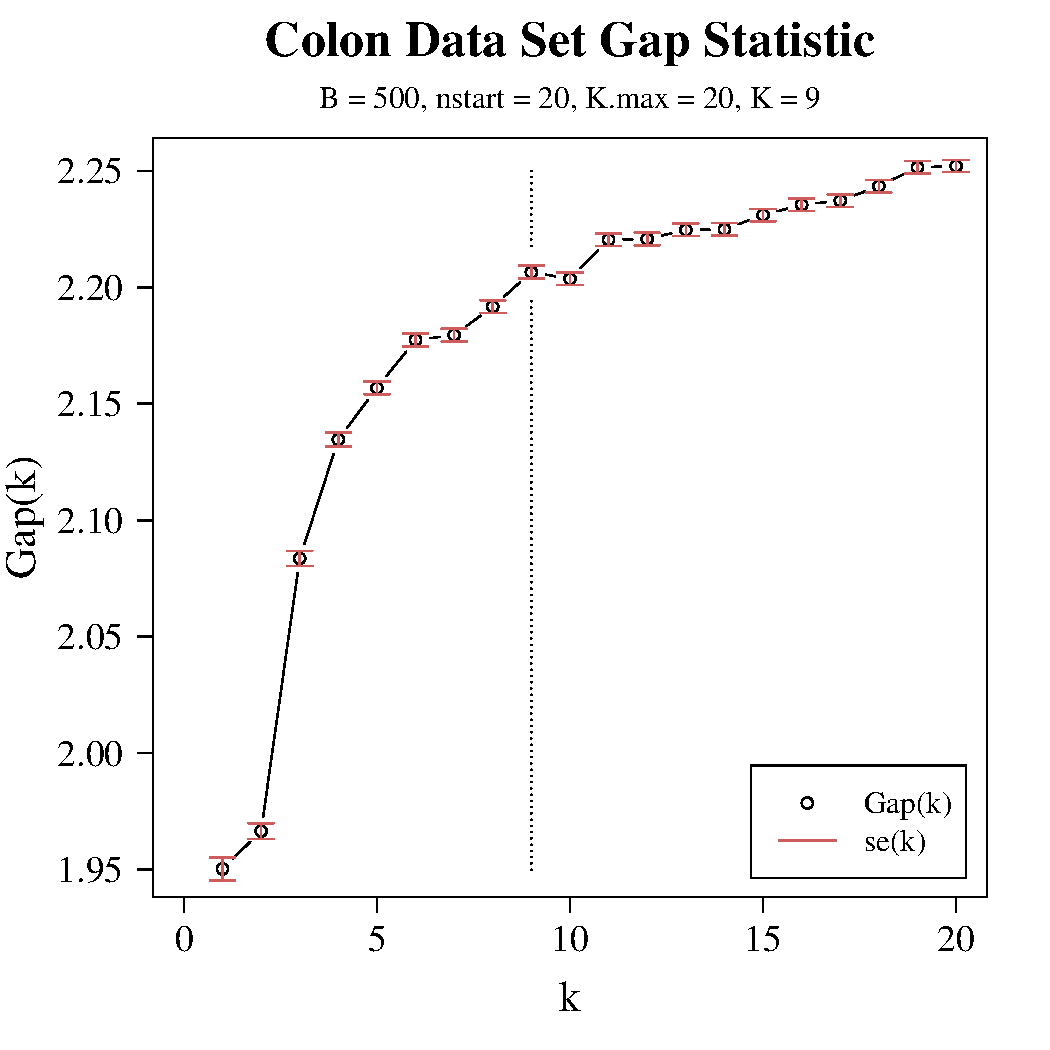
\includegraphics[width = 0.48\textwidth]{colon_gap_stat.pdf}
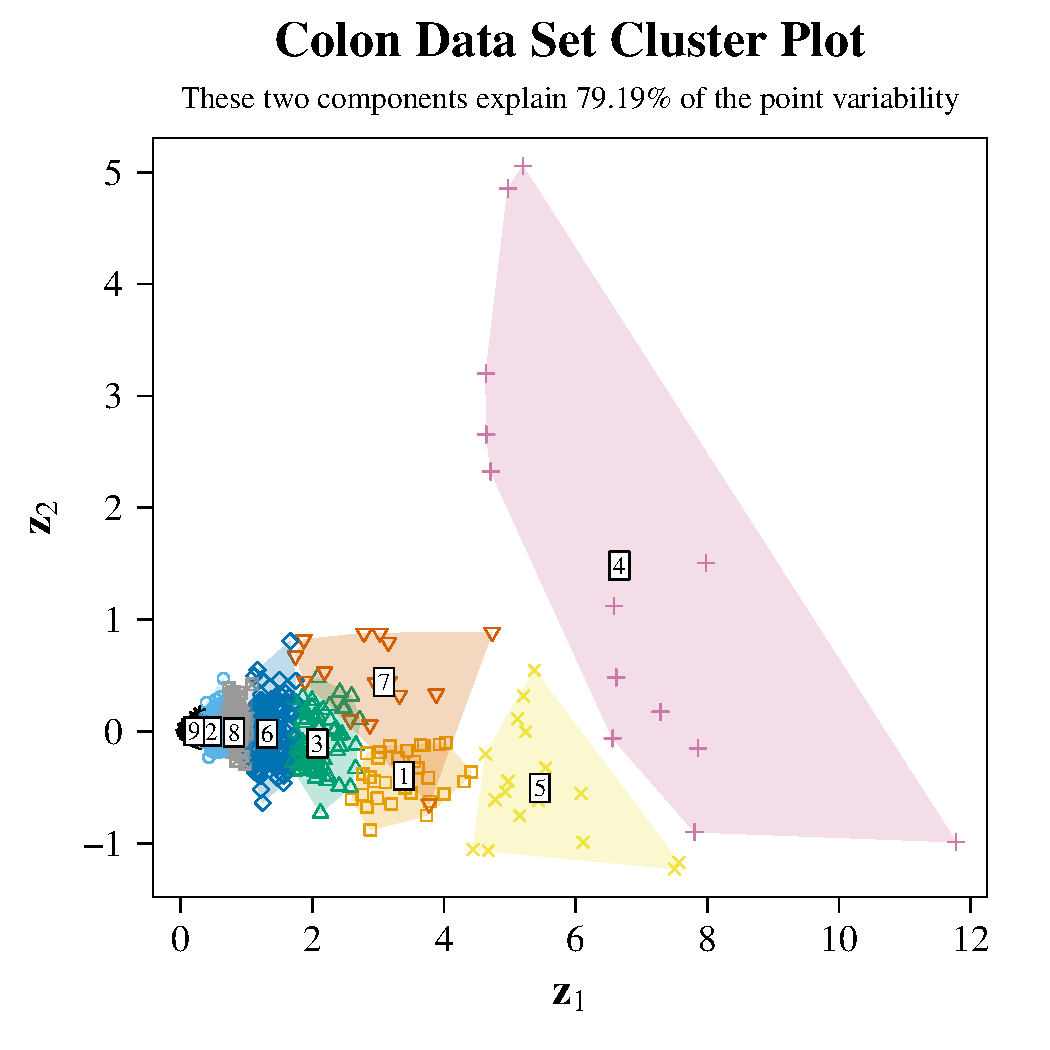
\includegraphics[width = 0.48\textwidth]{colon_clus_plot.pdf}

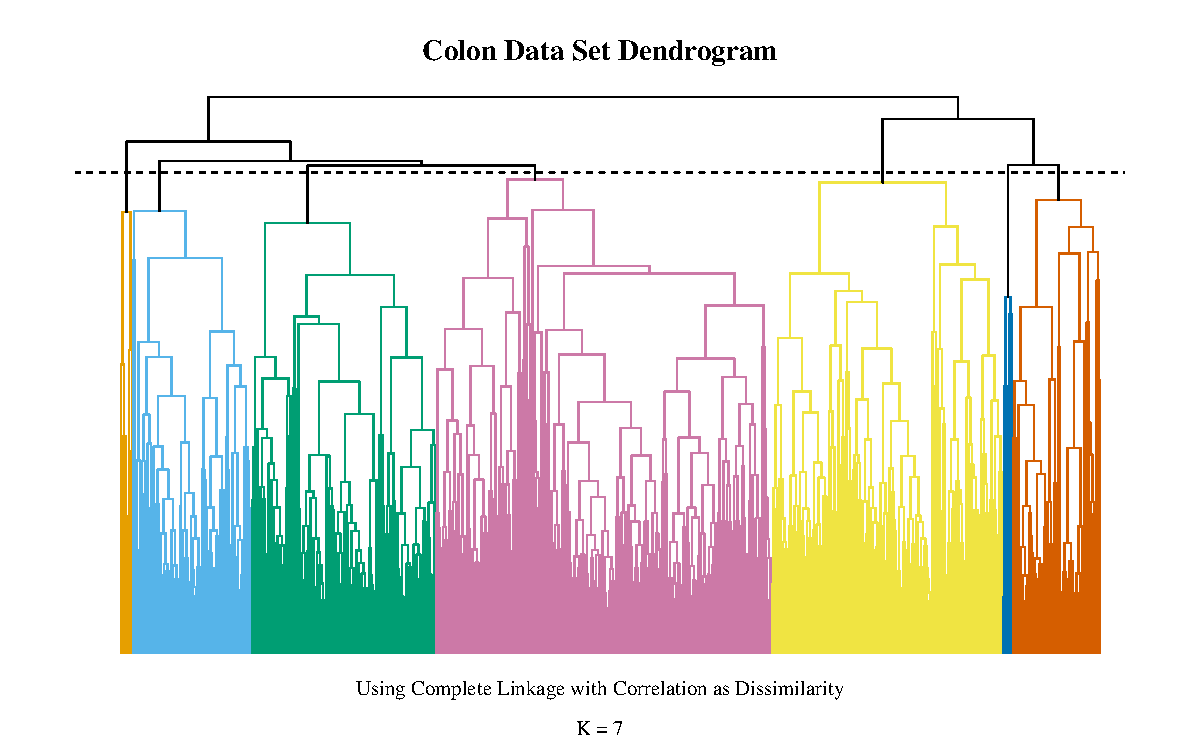
\includegraphics[width = \textwidth]{colon_den.pdf}
\caption{Clustering information for the colon data set.}
\label{colonclus}
\end{figure}

\newpage


\begin{figure}[ht]
\centering
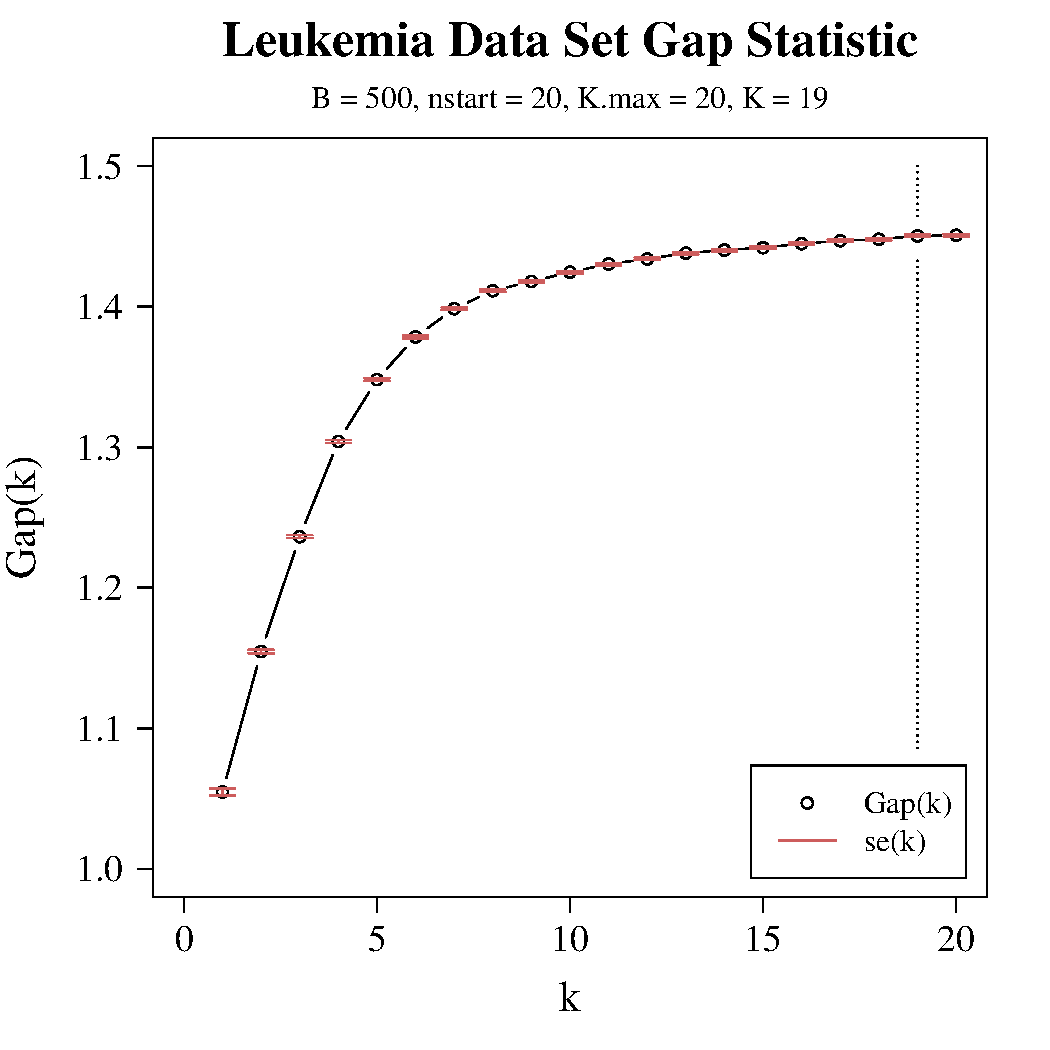
\includegraphics[width = 0.48\textwidth]{leuk_gap_stat.pdf}
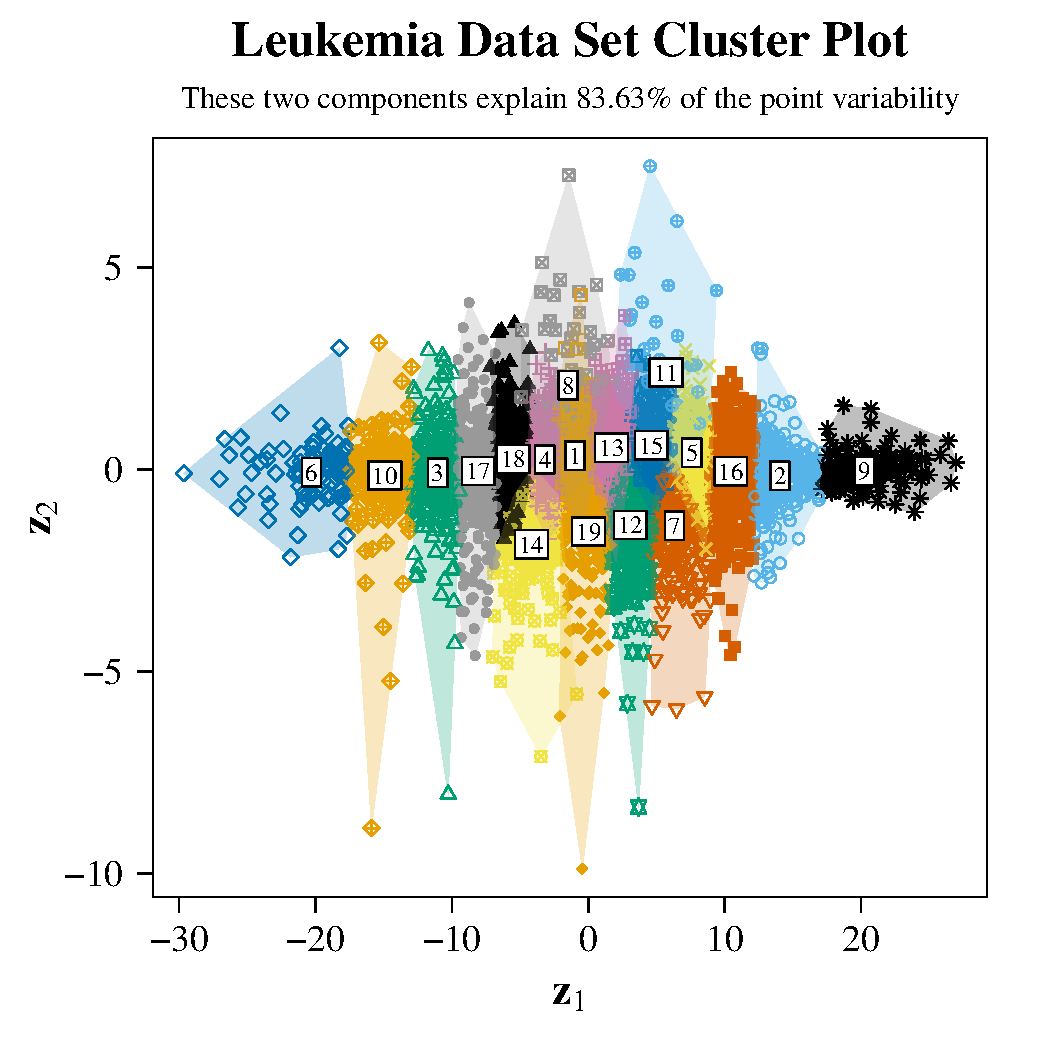
\includegraphics[width = 0.48\textwidth]{leuk_clus_plot.pdf}

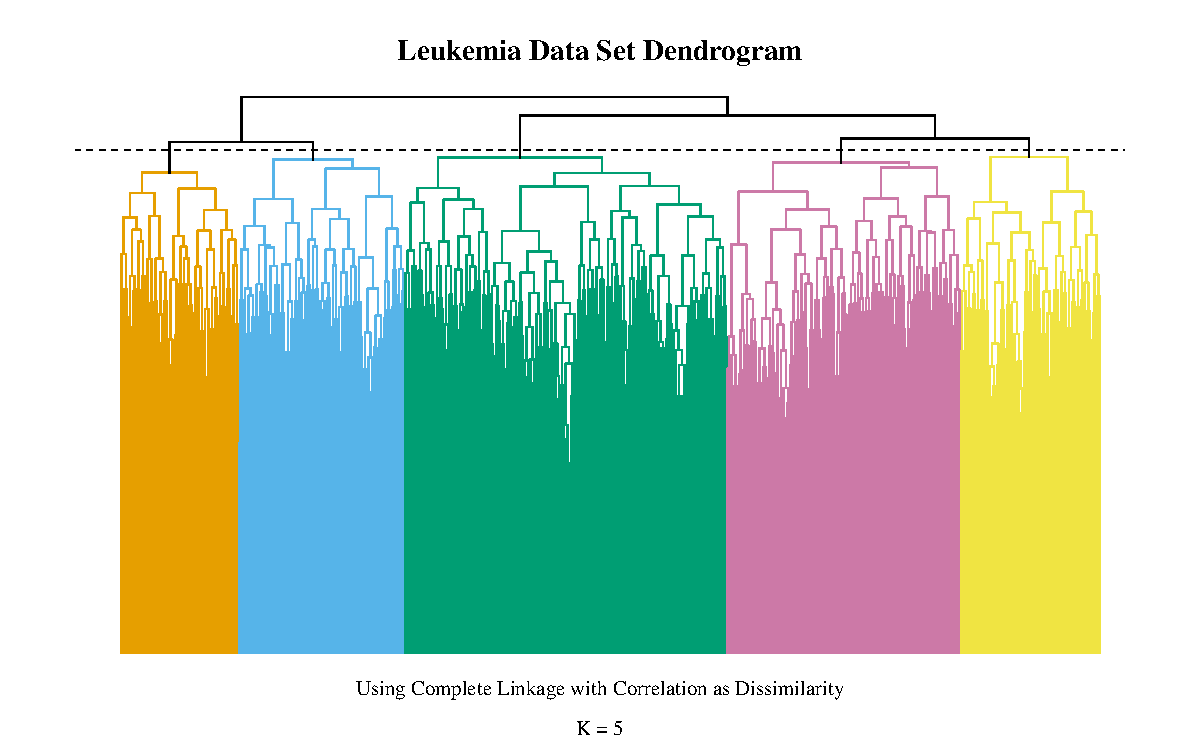
\includegraphics[width = \textwidth]{leuk_den.pdf}
\caption{Clustering information for the leukemia data set.}
\label{leukclus}
\end{figure}



\newpage

\begin{figure}[ht]
\centering
\includegraphics[width = 0.48\textwidth]{colon_kmeans_eigen.pdf}
\includegraphics[width = 0.48\textwidth]{colon_hclust_eigen.pdf}

\caption{Covariance eigenvalues for the colon data set. The left panel uses $K$-means clustering, while the right panel uses hierarchical clustering.}
\label{coloneigen}
\end{figure}


\end{document}

% https://stats.stackexchange.com/questions/220243/the-proof-of-shrinking-coefficients-using-ridge-regression-through-spectral-dec

% https://stats.stackexchange.com/questions/297280/ridge-regression-increase-in-lambda-leads-to-a-decrease-in-flexibilty/297475#297475

% https://stackoverflow.com/questions/9071020/compute-projection-hat-matrix-via-qr-factorization-svd-and-cholesky-factoriz

% https://www.cs.cornell.edu/courses/cs3220/2010sp/notes/svd.pdf

% https://intoli.com/blog/pca-and-svd/

% https://stats.stackexchange.com/questions/134282/relationship-between-svd-and-pca-how-to-use-svd-to-perform-pca

% https://stats.stackexchange.com/questions/297280/ridge-regression-increase-in-lambda-leads-to-a-decrease-in-flexibilty/297475#297475

% https://stats.stackexchange.com/questions/147880/is-pca-still-done-via-the-eigendecomposition-of-the-covariance-matrix-when-dimen